\addcontentsline{toc}{subsection}{Derivatives of Sine and Cosine}
\subsection*{Derivatives of Sine and Cosine}
Below is the graph of $y=\sin x$. Using the fact that $y'$ is the slope of the tangent line, make the graph of $y'$ for $y=\sin x$.
\begin{center}
    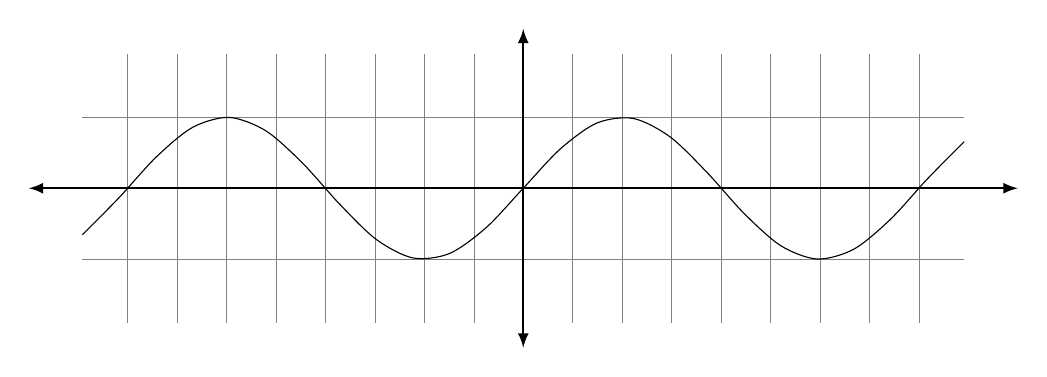
\begin{tikzpicture}[xscale=.8,yscale=.9]
          \draw[ystep=1,xstep=pi/4,style=help lines,] (-7,-1.9) grid (7,1.9);
          \draw[latex-latex, thick] (-7.85,0)--(7.85,0);
          \draw[latex-latex, thick] (0,-2.25)--(0,2.25);
          \draw[domain=-7:7, smooth] plot (\x, {sin(\x r)});
    \end{tikzpicture}
\end{center}

Similarly, attempt with the graph of $y=\cos x$.
\begin{center}
    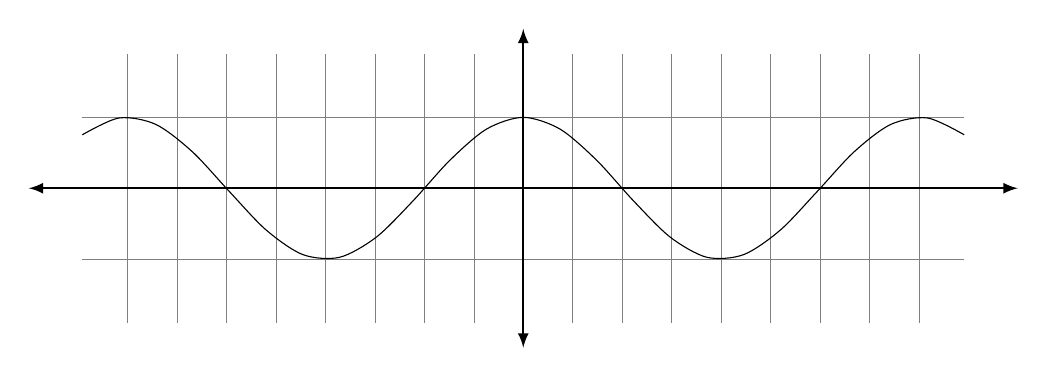
\begin{tikzpicture}[xscale=.8,yscale=.9]
          \draw[ystep=1,xstep=pi/4,style=help lines,] (-7,-1.9) grid (7,1.9);
          \draw[latex-latex, thick] (-7.85,0)--(7.85,0);
          \draw[latex-latex, thick] (0,-2.25)--(0,2.25);
          \draw[domain=-7:7, smooth] plot (\x, {cos(\x r)});
    \end{tikzpicture}
\end{center}
\vspace{.05cm}
\begin{tcolorbox}[title= DERIVATIVES OF SINE AND COSINE,colframe=black,sharp corners,colback=white,colbacktitle=white,coltitle=black,boxrule=1pt]

    \begin{align*}
        \frac{d}{dx}(\sin x) &= \hspace{1.5cm} & \frac{d}{dx}(\cos x) &= \hspace{1.5cm}
    \end{align*}
    \vspace{.05cm}
\end{tcolorbox}
\vspace{.15cm}
\noindent\textbf{Examples:}
Find the derivative of each of the following.
\begin{questions}
    \begin{minipage}{0.3\linewidth}
    \question $\displaystyle y=2\sin x$
    \end{minipage}
    \hfill
    \begin{minipage}{0.3\linewidth}
    \question $\displaystyle f(x)=\frac{-\sin x}{10}$
    \end{minipage}
    \hfill
    \begin{minipage}{0.3\linewidth}
    \question $\displaystyle u=x+\cos x$
    \end{minipage}
\end{questions}

\newpage
